\documentclass[11pt]{article}
\usepackage[a4paper,margin=2.2cm]{geometry}
\usepackage{fontspec}
\setmainfont[AutoFakeSlant=.2]{Noto Serif CJK SC}
\setsansfont{Noto Sans CJK SC}
\setmonofont{Noto Sans Mono CJK SC}
\XeTeXlinebreaklocale "zh"
\XeTeXlinebreakskip=0pt plus 1pt
\usepackage{amsmath,amssymb,graphicx,booktabs,array,float}
\usepackage[font=small,labelfont=bf]{caption}
\usepackage[numbers,sort&compress]{natbib}
\usepackage[dvipsnames]{xcolor}
\usepackage[colorlinks=true,linkcolor=MidnightBlue,citecolor=MidnightBlue,urlcolor=MidnightBlue]{hyperref}
\usepackage{fancyhdr,etoolbox}
\hypersetup{pdftitle={脉冲网络怎样用上先前的输入：门控双状态记忆},pdfkeywords={脉冲神经网络, 共享记忆}}
\renewcommand{\abstractname}{摘要}
\renewcommand{\refname}{参考文献}
\renewcommand{\figurename}{图}
\renewcommand{\tablename}{表}
\setlength{\parindent}{0pt}
\setlength{\parskip}{.5em}
\setlength{\emergencystretch}{2em}
\linespread{1.18}
\raggedbottom
\pagestyle{fancy}\fancyhf{}
\fancyhead[L]{\small GDSM · 共享记忆}
\fancyfoot[C]{\thepage}
\setlength{\headheight}{16pt}
\newcommand{\R}{\mathbb{R}}
\newcommand{\CE}{\operatorname{CE}}
\newcommand{\ind}{\mathbb{I}}
\newcommand{\pid}[1]{\ifstrequal{#1}{摘要}{}{\leavevmode\llap{\scriptsize\sffamily #1\hspace{.65em}}}\ignorespaces}
\newsavebox{\tablebox}
\title{\textbf{脉冲网络怎样用上先前的输入}\\[.3em]\large 门控双状态记忆（GDSM）}
\author{}\date{}

\makeatletter\renewcommand{\maketitle}{\begin{center}{\LARGE\@title\par}\end{center}}\makeatother
\begin{document}
\maketitle

\begin{abstract}

\pid{摘要} 听到词尾时，开头的声音已经过去，却仍有助于我们辨认这个词。双记忆通路（DMP）给每层脉冲神经元一份共享记忆，用它把先前的输入带到当前计算中。我们给这份记忆配上两种更新方式。候选状态逐帧跟随输入，稳定状态在写入门打开时接收候选内容，神经元同时读取两者。在语音命令数据集 SSC 上，两种模型采用相同的脉冲层，各用干净语音训练 200 轮。整词准确率从 DMP 的 72.34\% 提高到门控双状态记忆（GDSM）的 75.29\%。在另一组实验中，我们让同一个模型听完前半个词，再分别保留或清空它的稳定状态。只用后半段的输出分类，保留记忆让模型净多认对了 813 个词。在手势和逐像素输入的数字上，背景噪声接在原始输入之后，GDSM 也保住了更多正确答案。同等强度的噪声若贯穿手势动作，原 DMP 却认得更准。

\end{abstract}

\section{手是从哪一边过来的？}

\pid{1-P1} 一只手在空中画圆。顺时针和逆时针都要经过圆的最高点，单看手到了哪里，还分不清方向。要是记得它刚才从哪一侧过来，就知道它在往哪边转。事件相机把运动记录成一连串亮度变化。脉冲神经网络（SNN）依次收到这些事件。当它处理眼前这一步时，刚才那一段运动怎样才能派上用场？

\pid{1-P2} 一个漏积分发放（LIF）神经元本身就有记忆。它把刚收到的脉冲加到膜电位上，只是早先输入的影响会逐步衰减。Sun 等人研究双记忆通路时，关心的是怎样延长这段时间，同时控制芯片开销。给神经元增加循环连接，要存下更多权重。把脉冲延迟许多步再送达，又要为它们留出缓冲空间。他们采用的办法是让整层神经元共享一份低维记忆。神经元一边接收当前的输入电流，一边读取最近这段时间留下的信息。原文在逐像素图像和脉冲语音上检验了这种设计，并为快、慢两条通路设计了相应的硬件~\cite{dmp}。

\pid{1-P3} DMP 每来一帧就更新一次记忆。这样做的好处是，新动作一出现，记忆就开始跟着它变化。可是在画圆的例子里，网络还需要用到手先前的位置。工作记忆研究里也有类似的问题。Miller 等人先让猕猴看一张样本图，再依次呈现其他图片。后来的图片还要辨认，而最初那张图仍要留着，才能在它再次出现时作出反应~\cite{miller1996}。前额叶工作记忆的计算模型也讨论了在维持任务信息的同时，怎样控制下一次更新~\cite{millercohen,oreillyfrank}。

\pid{1-P4} 我们把 DMP 的共享记忆分成两份。一份随输入逐帧变化，称为候选状态。另一份有写入门，门打开时才接收候选内容，称为稳定状态。两份记忆都连回原来的脉冲层。这样，神经元可以一边跟踪手现在怎样运动，一边读取前几帧留下的信息。我们把这个结构称为门控双状态记忆（GDSM）。

\section{一层神经元怎样读写记忆}
\label{sec:method}

\begin{figure}[htbp]
\centering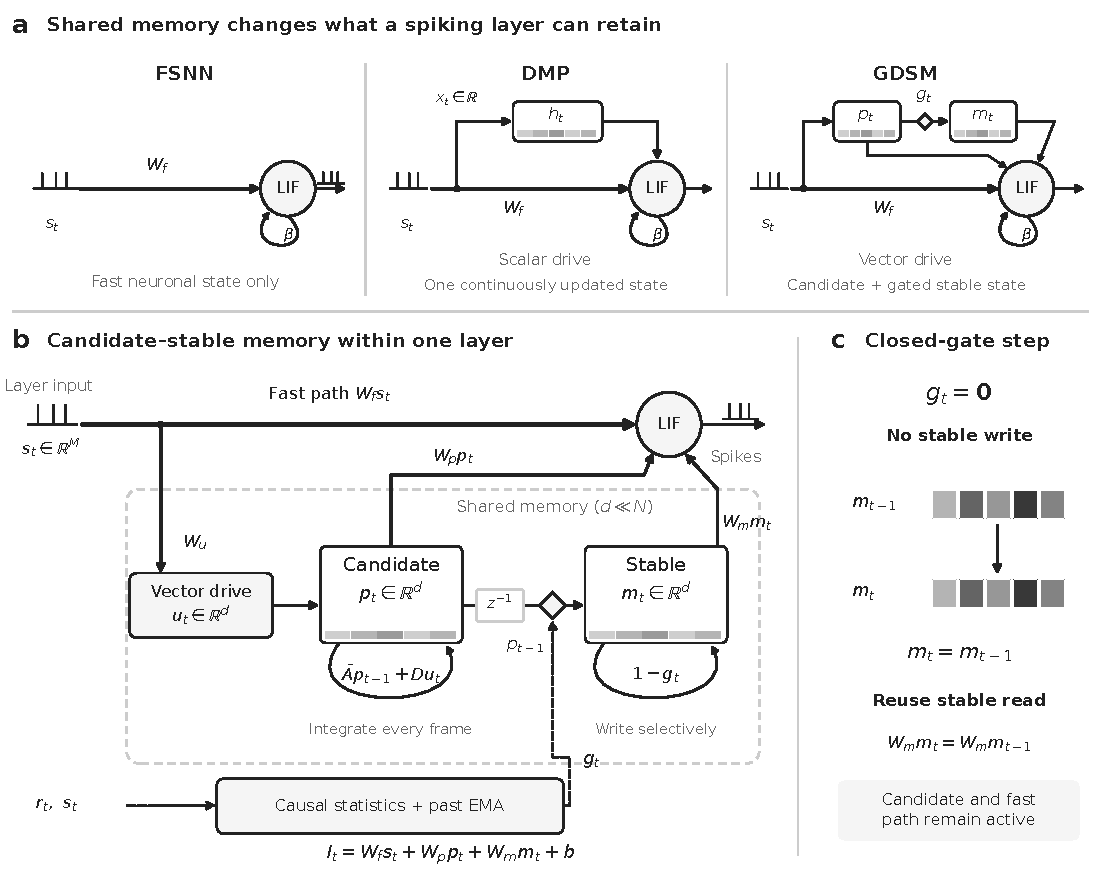
\includegraphics[width=0.93\linewidth]{figures/architecture.pdf}
\caption{共享记忆接回同一层 LIF 神经元。左边是 DMP。右边是 GDSM，候选状态的上一步输出经过菱形处的写入门进入稳定状态。两份状态各有一组读取权重，图中省略层号。}
\label{fig:architecture}
\end{figure}

\pid{2-P1} 先看语音模型的一层（图~\ref{fig:architecture}）。在一个具体配置里，每帧有 140 个输入通道，这一层有 128 个 LIF 神经元。原 DMP 把 140 个数投影成一个数，再用它推动一份 30 维记忆。这 30 个数由整层共享。每个神经元用自己的一组权重读取它们，得到一个记忆电流。因此 128 个神经元可以从同一份历史中读出不同的信息。下一层收到的是这 128 个神经元发出的脉冲，并维护自己的那份记忆。

\pid{2-P2} 先改记忆的入口。原来，两个不同的声音片段如果在那一个投影上取值相同，就会给慢记忆送进相同的输入。现在让模型学 30 组通道权重，每组各给出一个数。这样，一组可以对一种频带组合敏感，另一组可以对另一种组合敏感。这 30 个数推动候选状态 $p$ 逐帧更新。快通路仍然收到原来的 140 个通道。

\pid{2-P3} 接下来决定什么时候写。稳定状态 $m$ 也有 30 个数，每个坐标都有一个门值 $g$。门值为零就沿用旧值，为一就接收上一步的候选值，介于两者之间就按比例混合。下面是第 $l$ 层在第 $k$ 步的写入式，$\odot$ 表示对应坐标相乘。这里取上一步的候选值，给写入留出了一步时间。当前帧立刻改变候选状态，到下一步才可能经它进入稳定状态。

\begin{equation}
\begin{aligned}
 m^l[k]={}&(1-g^l[k])\odot m^l[k-1]\\
 &+g^l[k]\odot p^l[k-1].
\end{aligned}
\label{eq:stable}
\end{equation}

\pid{2-P4} 神经元同时读取两份状态。一份让它看到刚刚变化的输入，另一份提供上次写入后留下的内容。两份读取电流加上快通路的输入，一起决定这一步是否发放脉冲。关上写入门时，神经元照样读取稳定状态，候选状态也照样更新。

\pid{2-P5} 门只看当下和过去。传感器一帧全空时，整层停止向稳定状态写入。其余帧由模型根据活动强弱、变化和分布逐坐标决定。门控写入在循环网络中已有先例~\cite{lstm,gru}。这里一组门就能控制整层共享记忆的更新。附录~\ref{app:training} 给出完整的电流、门控和训练公式。

\section{前面的输入有没有参与分类}

\subsection{先让模型听完整个词}

\pid{3.1-P1} 先让模型辨认一个完整的事件。SHD 录的是人念的数字，SSC 录的是命令词，都在语音结束时分类。DVS Gesture 要从事件相机的记录中辨认动作。S-MNIST 把一张手写数字图逐个像素送入网络，PS-MNIST 则先按固定排列打乱像素顺序~\cite{shd,gesture,mnist}。每项任务各自训练模型。我们在已知的事件边界对整段类别分数取平均，比较同样骨干和训练安排下的 DMP 与 GDSM（表~\ref{tab:recognition}）。

\begin{table}[tbp]
\centering\small
\caption{事件结束时的干净分类准确率。从整段输出读取，无需等待。SSC 使用 200 轮干净训练。SHD、手势和两项图像任务使用各自微调后的模型。图像任务取三个训练种子的均值，另三项各用一组训练权重。差值按未舍入的准确率计算。}
\label{tab:recognition}
\begin{tabular}{lrrrr}
\toprule
任务 & 测试样本 & DMP（\%） & GDSM（\%） & 差值（百分点）\\\midrule
SHD & 2,264 & 89.80 & 90.33 & $+0.53$\\
SSC & 20,382 & 72.34 & 75.29 & $+2.95$\\
DVS Gesture & 264 & 86.74 & 86.74 & $0.00$\\
S-MNIST & 10,000 & 94.39 & 96.42 & $+2.03$\\
PS-MNIST & 10,000 & 89.00 & 89.63 & $+0.63$\\
\bottomrule
\end{tabular}
\end{table}

\pid{3.1-P2} 五项任务里，手势的干净准确率相同，其余四项的差值在 0.53 到 2.95 个百分点之间。逐像素图像在训练早期就能看出差别。以 S-MNIST 为例，第 5 轮时 DMP 的干净验证准确率为 82.64\%，GDSM 为 92.12\%，到训练结束两者的差距已经缩小。图~\ref{fig:training} 给出验证曲线，其中 SSC 曲线来自单独的混合训练配方。

\begin{figure}[htbp]
\centering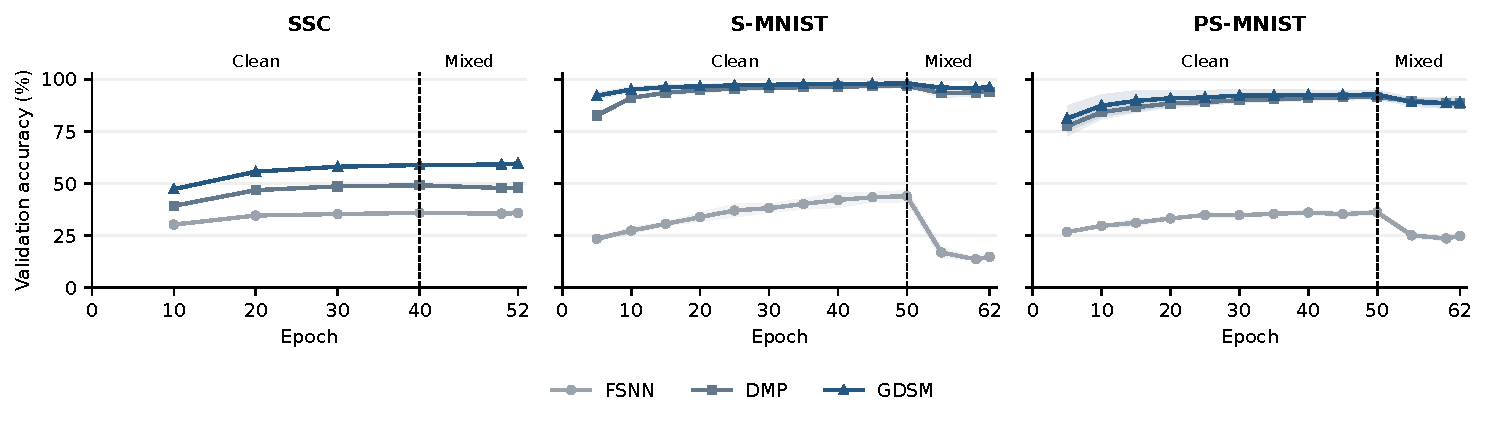
\includegraphics[width=\linewidth]{figures/training-curves.pdf}
\caption{训练中对干净验证样本的识别。虚线标出从干净训练转入混合训练的时刻。点表示实际记录的轮次。SSC 使用 40+12 轮配方。两项图像任务给出三个训练种子的均值和一个标准差。}
\label{fig:training}
\end{figure}

\pid{3.1-P3} SSC 的整词结果还可以从两方面看。两种模型都用两层各 256 个神经元，在相同样本上更新 59,000 次。DMP 有 116,913 个可训练参数，GDSM 有 127,639 个。把共享记忆换成双状态后，准确率提高了 2.95 个百分点。再取这个已经训练好的 GDSM，只关闭两个隐藏层从稳定状态读取电流的权重，保留偏置和其余计算，准确率从 75.29\% 降到了 23.17\%。可见正常听词时，神经元已经在使用这份记忆。要知道它用到了多久以前的信息，还可以做一次更有针对性的实验。

\subsection{同一个词，听到一半时清空一次记忆}

\pid{3.2-P1} 把一个词的 250 帧分成前后两半。模型听完前 125 帧后，我们复制它此时的全部状态。两份副本接着听完全相同的后半个词。唯一的改动，是在其中一份里把两层的稳定状态清零一次。候选状态、膜电位和门控历史都照常带入后半段，从第 126 帧起也照常写入。最后只取后 125 帧的类别分数判定原词。前半段对类别的投票由此排除在评分之外。

\pid{3.2-P2} 这个实验使用另一组已训练的 SSC 权重（每层 128 个神经元，先干净训练 200 轮，再混合训练 12 轮）。在 20,382 条测试语音上，两份副本用后半段的输出分别认对了 32.83\% 和 28.84\%（保留和清零）。两者净差 813 个词，即 3.99 个百分点。若只在后半段叠加背景脉冲，同样的对照是 17.73\% 和 15.33\%，净差 489 个词。这是一个词还在播放时发生的差别。两次听到的后续声音相同，带着前半段形成的状态继续听，后半段的判断就更准一些。

\section{用噪声看清记忆的作用}

\subsection{手还在动，还是动作已经做完了}

\pid{4.1-P1} 换到手势，两种模型在干净输入上恰好打成平手。我们做了两次测试。第一次，从动作开始到结束一直叠加背景事件，动作一结束就分类。第二次，让模型先看完干净动作，再送入 80 帧背景事件，只用最后 20 帧的输出回答刚才是什么动作。两次都使用按训练数据标定的同一平均噪声强度。前一次要求在噪声中看清动作，后一次可以单独观察已经得到的信息还能起多久的作用。

\pid{4.1-P2} 噪声伴着动作出现时，DMP 认对了 75.76\%，GDSM 认对了 64.39\%。把噪声移到动作之后，结果变成 24.24\% 和 46.59\%。再取两个模型原来都认对的 224 段手势逐段比较。在动作期间加噪，GDSM 比 DMP 净少认对 25 段。在动作之后加噪，它净多认对 58 段。同一对模型，同一批动作，改变干扰的时机就改变了两者的相对表现（图~\ref{fig:paired}）。

\begin{figure}[htbp]
\centering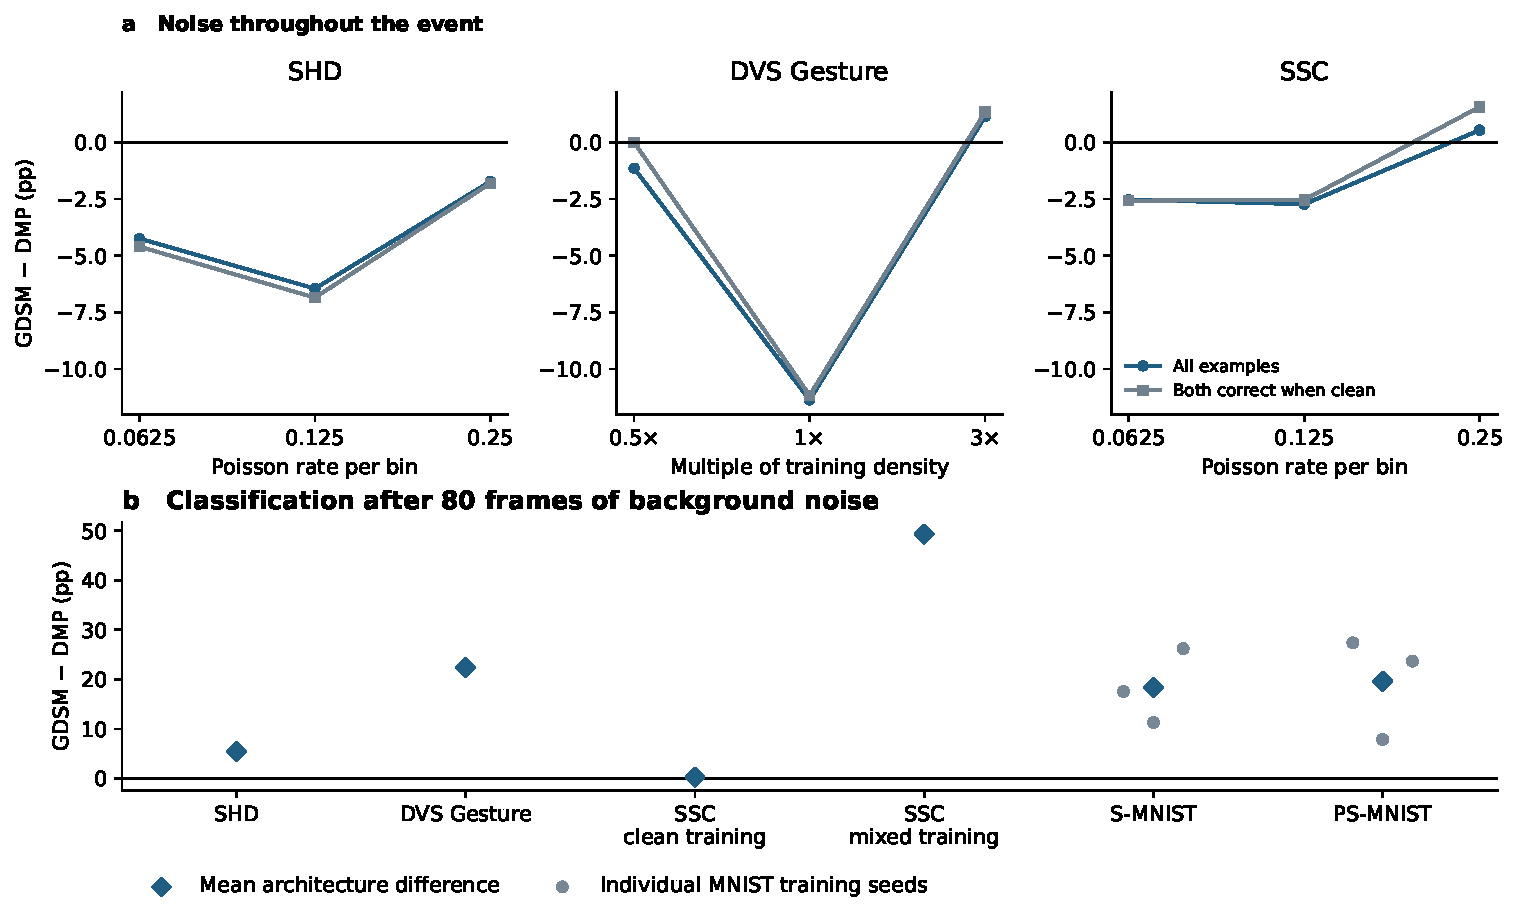
\includegraphics[width=0.95\linewidth]{figures/paired-effects.pdf}
\caption{GDSM 与 DMP 的准确率差（百分点）。（a）噪声从事件开始叠加到结束，分别在全部样本和两个模型在干净条件下都认对的样本上评分。（b）事件后追加 80 帧背景噪声，取最后 20 帧输出。菱形为架构差值，圆点为图像任务各个训练种子的结果。各任务的噪声单位见附录~\ref{app:training}。}
\label{fig:paired}
\end{figure}

\pid{4.1-P3} 在两项语音任务上，背景脉冲贯穿整词也会削弱 GDSM 的表现。每通道每帧平均叠加 0.125 个事件时，SHD 的 DMP 和 GDSM 分别为 52.56\% 和 46.11\%。同一强度下，表~\ref{tab:recognition} 中干净训练的 SSC 模型分别为 12.14\% 和 9.42\%。另一组接触过干扰的 SSC 模型在低噪声下保有优势，噪声越强，优势越小，到 0.25 时 DMP 为 14.43\%，GDSM 为 9.77\%（图~\ref{fig:speech}）。一份记忆能把已有线索留住多久，和它能从一开始就混着噪声的信号里读出多少线索，是两个可以分别测量的问题。

\begin{figure}[htbp]
\centering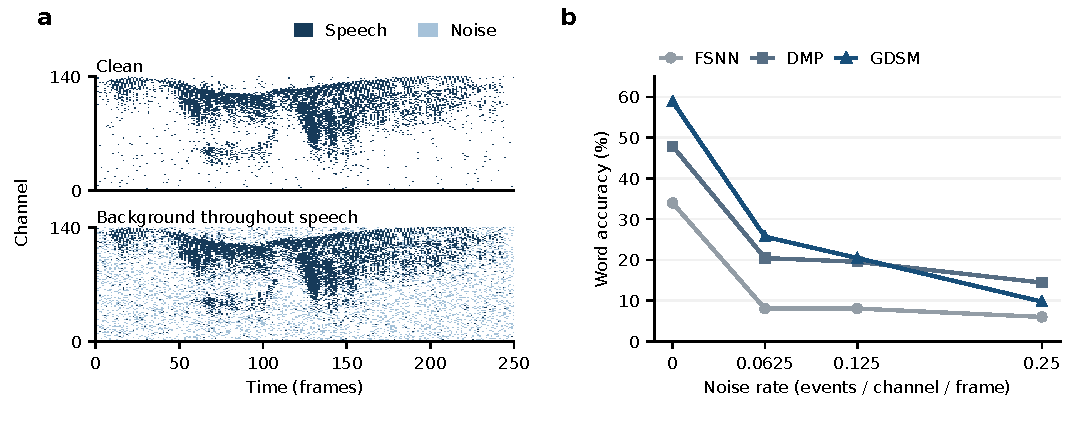
\includegraphics[width=\linewidth]{figures/ssc-speech.pdf}
\caption{SSC 的 40+12 轮混合训练配方。（a）同一条语音，上图为干净脉冲，下图为全程叠加均值 0.25 的泊松背景后得到的输入。（b）三个模型在相同的 20,382 条测试语音上、用整词输出得到的准确率。FSNN 为只有快通路的脉冲网络。}
\label{fig:speech}
\end{figure}

\subsection{让线索离开输入，再读一次}

\pid{4.2-P1} 在像素序列上也能做同样的检查。每个模型都已经看完组成数字的 784 个像素，再输入 80 帧噪声。普通扫描顺序下，DMP 和 GDSM 的准确率分别为 40.53\% 和 58.87\%。打乱像素顺序后，分别为 26.33\% 和 45.96\%，都是三个训练种子的均值。把测试延长到训练中没有见过的 160 帧静默，普通顺序下仍有 78.68\% 的图像能从 GDSM 的末段输出认出，DMP 为 8.69\%。打乱顺序时两者分别为 56.43\% 和 14.12\%。图~\ref{fig:retention} 给出了随间隔长度变化的过程。语音任务的绝对准确率有时很低。以表~\ref{tab:recognition} 的 SHD 模型为例，80 帧噪声后是 4.95\% 和 10.29\%（DMP、GDSM）。

\pid{4.2-P2} 网络怎样训练，会影响它怎样使用这条通路。只用干净词训练 200 轮的 SSC 模型，在词后追加 80 帧噪声时，DMP 为 2.96\%，GDSM 为 3.22\%，都接近 35 类任务的随机水平。在另一组 40+12 轮的配方里，训练会要求模型在干扰过后仍回答原词。追加 120 帧噪声后，DMP 为 3.91\%，GDSM 为 52.79\%。两组配方的骨干宽度和输入聚合方式也不同。若只跟踪后一个配方里同一 GDSM 的学习过程，进入混合训练前它在这一条件下是 11.47\%，混合训练后才达到 52.79\%。

\begin{figure}[htbp]
\centering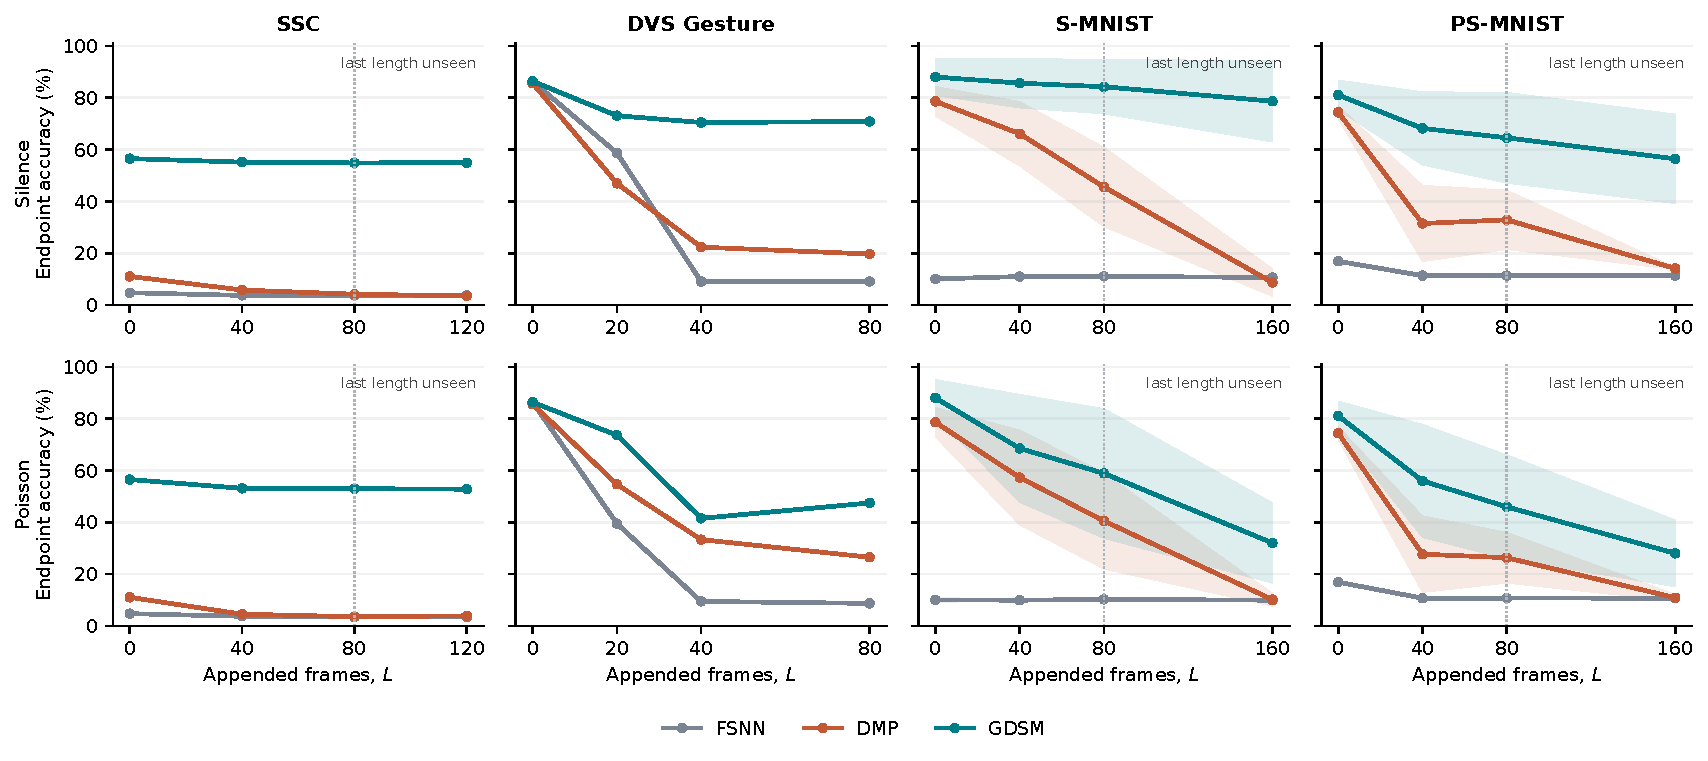
\includegraphics[width=\linewidth]{figures/retention.pdf}
\caption{在原始事件之后读取类别。横轴为追加的帧数，所有点都只取最后 20 帧的输出，零点为干净事件的末段。竖虚线标出最长训练间隔（如有更长的测试间隔）。手势噪声结果平均三次采样，图像任务的阴影为训练种子间的一个标准差。}
\label{fig:retention}
\end{figure}

\pid{4.2-P3} SHD 还可以用来追问，增益有多少与记忆入口有关。我们用同一套带辅助监督的配方，训练两种参数量几乎相同的模型。一种先扩到 30 个数又压回 1 个数，再写入记忆。另一种把 30 个数都送入候选状态。只读稳定状态时，干净词末的类别准确率由 69.57\% 升到 81.05\%。让整个网络在 80 帧干扰后识别，静音和噪声两种条件的平均准确率由 59.76\% 升到 66.70\%（附录~\ref{app:shd}）。写入门能保留下来的东西，首先取决于记忆入口送进来了什么。

\section{多一份记忆要花多少计算}

\pid{5-P1} DMP 的一个优点是记忆由整层共享，我们也想保留这个优点。额外的计算来自向量输入投影、写入门和稳定状态的读取。如果一步里所有写入门都关闭，稳定状态没有变化，上一步算好的读取电流便可以直接复用。在干净手势上，按整个网络统计，DMP 平均每例需要 63.212 百万次有效乘加，使用缓存的 GDSM 需要 67.196 百万次，增加 6.30\%（图~\ref{fig:hardware}）。追加 80 帧静音时，缓存省下了 GDSM 自身全网乘加的 1.18\%。

\pid{5-P2} 我们在原 DMP 的 Chisel 工程中实现了这条记忆通路，用一个训练好的层的权重重放 944 步输入。定点电路的 117,056 个受检数值逐个与整数参考实现一致。重放检验的是记忆核按什么次序计算、每个值算得对不对。整网乘加数是另一项估算，芯片的实际能耗仍要测量。

\begin{figure}[htbp]
\centering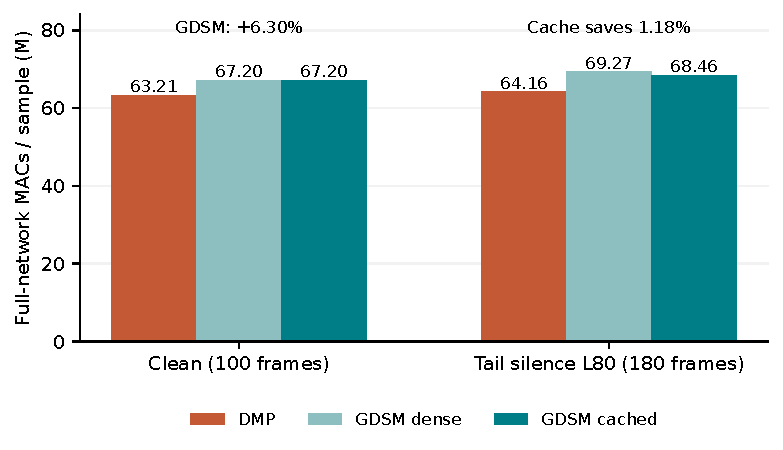
\includegraphics[width=\linewidth]{figures/full-network-macs.pdf}
\caption{DVS Gesture 每段测试动作的全网有效乘加数，取 264 段的平均值。Dense 为每步重新计算，cached 允许复用稳定读取。纵轴从零开始，单位为百万次乘加。}
\label{fig:hardware}
\end{figure}

\section{回到正在发生的动作}

\pid{6-P1} 手走到圆的最高点时，走过的那一段还应该对当前判断有用。原 DMP 给过去的输入留了一条通道。我们的改动是让这条通道里的两份状态可以按不同的节奏更新。词中清零实验直接说明了这件事。同一个模型听到同样的后半个词，保留前半段留下的稳定状态，就能多认对一些词。至于它留下的究竟是哪些音素或运动线索，还可以继续追踪。

\pid{6-P2} 后续输入的内容决定了这份记忆能帮上什么忙。手势已经看清，背景事件才出现，稳定状态能让刚才的线索多起一段时间的作用。背景事件从动作一开始就混在其中，两种通路读到的线索都可能失真，在我们测的中档噪声下，原 DMP 反而认出了更多手势。下一步值得追问的是，在动作还没结束时，哪些新证据值得写进稳定状态，哪些先留在候选状态里就够了。

\paragraph{数据与代码}

\pid{6-P3} 数据集开放获取~\cite{shd,gesture,mnist}。代码、逐样本预测和硬件重放记录见 \url{https://github.com/Veirsune/Dual_memory_pathways}。

\input{main.bbl}
\appendix

\section{门控、训练和计算口径}
\label{app:training}

\pid{A-P1} 沿用原 DMP 的记号，第 $k$ 步进入第 $l$ 层的输入为 $s^{l-1}[k]\in\R^M$，该层 $N$ 个神经元的膜电位为 $u^l[k]\in\R^N$。DMP 的 $x^l[k]$ 是标量驱动，$m^l[k]\in\R^d$ 是共享记忆。输入映射为 $f_x$，固定的 $\bar A\in\R^{d\times d}$ 与 $\bar B\in\R^{d\times1}$ 来自离散 Legendre 记忆单元~\cite{dmp,lmu}。

\begin{equation}
\begin{aligned}
 x^l[k]&=f_x(W_x s^{l-1}[k]+b),\\
 m^l[k]&=\bar A m^l[k-1]+\bar B x^l[k] .
\end{aligned}
\label{eq:dmp}
\end{equation}

\pid{A-P2} GDSM 将投影 $W_x$ 从一行扩为 $d$ 行，用向量 $\mathbf{x}^l[k]$ 驱动候选状态 $p^l[k]$。实现中的 $f_x$ 为 ReLU。代码里另有一个固定的正对角缩放，可由 ReLU 的正齐次性并入 $W_x$ 和 $b$。语音的 Legendre 记忆窗 $\theta=40$，手势和图像为 300。用状态压缩最近输入的思路也见于其他线性记忆和状态空间模型~\cite{hippo,s4}。

\begin{equation}
\begin{aligned}
 \mathbf{x}^l[k]&=f_x(W_x s^{l-1}[k]+b),\\
 p^l[k]&=\bar A p^l[k-1]+\bar B\odot \mathbf{x}^l[k] ,
\end{aligned}
\label{eq:candidate}
\end{equation}

\pid{A-P3} 稳定状态按式~\eqref{eq:stable} 写入。快输入提供 $I^l[k]$，候选与稳定状态各自投影后提供 $I_m^l[k]$。两股电流及合并后的偏置共同驱动 LIF 神经元。每条新序列的状态从零开始，插入间隔时状态连续。

\begin{equation}
\begin{aligned}
 I^l[k]&=W_f s^{l-1}[k],\\
 I_m^l[k]&=W_p p^l[k]+W_m m^l[k].
\end{aligned}
\label{eq:read}
\end{equation}

\pid{A-P4} 局部门的输入 $f^l[k]$ 包含归一化平均活动、平均活动的绝对变化、方差和非零位置比例。历史值按 $e^l[k]=\rho e^l[k-1]+(1-\rho)f^l[k]$ 更新，$\rho=0.8$。式~\eqref{eq:gate} 中，$q^l[k]$ 是一个小型感知机按当前原始输入的统计特征及其历史均值给出的逐维二值许可，$s^0[k]$ 是当前传感器帧。阈值 $\varepsilon=0.02$。原始帧全空、局部门低于阈值或没有许可，均可使相应写入精确为零。若连续 80 步写入系数都为 0.02，旧状态的直接贡献系数就只剩 $0.98^{80}\approx0.20$，因此精确关门和保持小幅写入有不同的后果。

\begin{equation}
\begin{aligned}
 \hat g^l[k]&=\sigma\!\left(W_g[f^l[k];e^l[k-1]]+b_g\right),\\
 g^l[k]&=\ind[\|s^0[k]\|_1>0]\,
       \hat g^l[k]\\
 &\quad\odot\ind[\hat g^l[k]\ge\varepsilon]\odot q^l[k] .
\end{aligned}
\label{eq:gate}
\end{equation}

\pid{A-P5} 前向计算使用硬门，反向计算使用 sigmoid 代理梯度~\cite{surrogate,spikingjelly}。局部门初始权重为零、偏置为 $\log(0.95/0.05)$，许可网络的输出层初始权重为零、偏置为 $+2$。与逐神经元学习门控或时间常数的模型~\cite{glif,tclif}相比，这里门的维度只随共享记忆大小变化。根据输入调节状态更新也见于选择性状态空间模型~\cite{mamba}。

\pid{A-P6} 普通整词训练对 $T$ 帧的平均类别分数 $o[k]$ 计算交叉熵。混合训练额外取最后 $K=20$ 帧的平均分数，两个损失等权（$\lambda=0.5$，式~\eqref{eq:loss}），目标都是原类别 $y$。这让模型能从干扰末段的输出得到学习信号。事件边界用于分帧和评分，写入门只接收输入特征。两种层内记忆通过任务误差训练。附录~\ref{app:shd} 单独注明了使用辅助监督的 SHD 实验。

\begin{equation}
\begin{aligned}
\mathcal L={}&(1-\lambda)\CE\!\left(\frac1T\sum_{k=1}^{T}o[k],y\right)\\
 &+\lambda\CE\!\left(\frac1K\sum_{k=T-K+1}^{T}o[k],y\right),
\end{aligned}
\label{eq:loss}
\end{equation}

\begin{table}[H]
\centering\small
\caption{训练与测试规模。$T_0$ 是原始帧数，$d$ 是每份共享状态的维度。最后一列为干净训练轮数加微调轮数。手势在 50 轮内按验证结果选择起点。SSC 的 200+12 配方用于词中清零实验。}
\label{tab:protocol}
\begin{lrbox}{\tablebox}\begin{tabular}{lrrrrll}
\toprule
任务 & 训练 / 验证 / 测试 & 类别数 & $T_0$ & $d$ & 骨干网络 & 干净+混合轮数\\
\midrule
SHD & 8,156 / -- / 2,264 & 20 & 100 & 30 & $140\to128\to128\to20$ & $200+30$\\
SSC & 75,466 / 9,981 / 20,382 & 35 & 250 & 10 & $140\to256\to256\to35$ & $200+0$\\
SSC & 75,466 / 9,981 / 20,382 & 35 & 250 & 10 & $140\to128\to128\to35$ & $200+12$\\
SSC & 75,466 / 9,981 / 20,382 & 35 & 250 & 30 & $140\to128\to128\to35$ & $40+12$\\
DVS Gesture & 901 / 176 / 264 & 11 & 100 & 40 & Conv32--Conv64--FC256--11 & $50+20$\\
S-MNIST & 54,000 / 6,000 / 10,000 & 10 & 784 & 40 & $1\to200\to200\to10$ & $50+12$\\
PS-MNIST & 54,000 / 6,000 / 10,000 & 10 & 784 & 40 & $1\to200\to200\to10$ & $50+12$\\
\bottomrule
\end{tabular}\end{lrbox}
\ifdim\wd\tablebox>\linewidth\resizebox{\linewidth}{!}{\usebox{\tablebox}}\else\usebox{\tablebox}\fi
\end{table}

\pid{A-P7} 表~\ref{tab:recognition} 中 SHD 的两种架构从同一个预训练 DMP 开始，在 8,156 条训练语音上按相同顺序和类别损失微调 30 轮（种子 301）。SSC 的 256 宽模型用种子 42、batch 256、初始学习率 0.01 的 Adam，按干净验证集选模。原初始学习率 0.1 下，两者的干净测试准确率是 60.21\% 和 67.68\%，选中的 DMP 在抽查的 2,048 条验证语音上两层记忆驱动均为零。词中清零用 128 宽的独立模型，训练种子为 42。两种 200 轮配方均把相邻五个听觉通道求和。40+12 轮 SSC 配方用最大池化、batch 512、种子 801，干净与混合阶段的 AdamW 学习率分别为 0.003 和 0.001，两个阶段都使用式~\eqref{eq:loss}。

\pid{A-P8} 手势使用受试者 1--19 训练、20--23 验证、24--29 测试，输入为 100 帧双极性 $32\times32$ 图像。20 轮混合训练用种子 701。MNIST 的训练与验证集分层抽样，三次训练使用种子 42--44 和同一像素排列。18 个 MNIST 模型均在正式测试前冻结。SHD、SSC 的开发和评估时间线，以及各组的样本划分和选模过程，见随文的实验记录。

\pid{A-P9} 整段叠加测试的语音噪声是独立泊松计数，均值为每通道每帧 0.0625、0.125 或 0.25。词后 80 帧测试采用其中的 0.25。手势在动作期间测试训练平均活动密度的 0.5、1 和 3 倍，配对的动作后测试用 1 倍。图像间隔的泊松率为 0.1，数值截到 $[0,1]$。两个模型在各自条件下看到同一次采样。手势逐例分析每条件一次采样，间隔长度曲线则平均三次采样。语音和图像混合训练的间隔为 40 或 80 帧，手势另含 20 帧。在事件中间插入间隔会延长序列，间隔后原事件继续。叠加噪声时原事件的时长不变。

\paragraph{硬件}\label{app:hardware}

\pid{A-P10} 记忆核使用有符号的 24 位 Q11.12 运算。给定 4 个输入和 32 个读取输出，$d=10/30$ 时 DMP 的局部更新为 43/63 周期，GDSM 为 136/216 周期，全门关闭并使用缓存时为 104/184 周期。训练权重重放包含 784 个像素步、80 帧静默和 80 帧噪声，测试一个真实 $d=40$ 层的四个读取坐标，缓存使执行周期由 188,800 降至 185,528。这些是记忆核的时序和整数核验数据。

\section{拆开看输入投影和写入门}
\label{app:shd}

\pid{B-P1} 这里使用 SHD 的独立机制对照。容量实验在同一训练配方下改变输入投影，包含稳定状态辅助分类损失（权重 1.0）以及依据干扰位置给出的门控监督。表~\ref{tab:capacity} 中宽标量模型经 $M\to d\to1$ 压缩，向量模型保留 $d$ 个输入，两者使用相同的读取和保护方式。$d=30$ 时向量模型还少 62 个参数，可读出的类别信息却更多。

\begin{table}[H]
\centering\small
\caption{SHD 投影对照，种子 501。“存入”取干净词末稳定状态的辅助分类准确率，“保留”取整个脉冲网络在 80 帧静音和噪声后的平均准确率。}
\label{tab:capacity}
\begin{lrbox}{\tablebox}\begin{tabular}{rlrrr}
\toprule $d$ & 驱动 & 参数量 & 存入（\%） & 保持（\%）\\\midrule
10 & 标量 & 45,050 & 48.19 & 40.15\\
10 & Wide scalar & 47,502 & 56.67 & 47.46\\
10 & 向量 & 47,480 & 68.24 & 51.88\\\addlinespace
30 & 标量 & 57,410 & 68.82 & 52.65\\
30 & Wide scalar & 65,302 & 69.57 & 59.76\\
30 & 向量 & 65,240 & 81.05 & 66.70\\
\bottomrule
\end{tabular}\end{lrbox}
\ifdim\wd\tablebox>\linewidth\resizebox{\linewidth}{!}{\usebox{\tablebox}}\else\usebox{\tablebox}\fi
\end{table}

\pid{B-P2} 写入监督实验从匹配的起始权重微调 30 轮，使用三个种子 501--503，各组均保留辅助类别损失。$d=30$ 时，仅靠类别监督并对空帧关门，静音后的准确率为 67.82\%，噪声后为 60.16\%。再提供干扰位置训练写入门，噪声结果为 60.81\%（表~\ref{tab:supervision}）。若把同样总强度的背景脉冲集中到相邻 28 个通道，空帧关门模型的噪声后准确率降到 6.91\%。改变噪声落在哪些频带，也会改变记忆能留下什么。

\begin{table}[H]
\centering\small
\caption{SHD 写入门对照，准确率（\%）为三个微调种子的均值与标准差。静音与噪声均为 80 帧，新词一栏读取下一个词。}
\label{tab:supervision}
\begin{lrbox}{\tablebox}\begin{tabular}{rlrrrr}
\toprule $d$ & 训练方式 & 干净 & 静音 L80 & 噪声 L80 & 新词\\\midrule
10 & 类别监督 & $85.62\pm2.06$ & $31.38\pm3.19$ & $41.64\pm9.83$ & $73.28\pm2.51$\\
10 & 类别监督 + 零输入关闭 & $86.31\pm1.11$ & $58.42\pm4.47$ & $46.29\pm8.23$ & $72.97\pm1.60$\\
10 & 类别监督 + 零输入关闭 + 门控标签 & $86.10\pm1.85$ & $60.38\pm4.03$ & $53.47\pm4.17$ & $69.05\pm1.82$\\\addlinespace
30 & 类别监督 & $87.38\pm0.98$ & $29.52\pm6.19$ & $56.96\pm12.77$ & $75.89\pm1.27$\\
30 & 类别监督 + 零输入关闭 & $87.99\pm0.87$ & $67.82\pm5.48$ & $60.16\pm8.76$ & $75.63\pm1.59$\\
30 & 类别监督 + 零输入关闭 + 门控标签 & $87.99\pm0.19$ & $66.84\pm7.17$ & $60.81\pm13.50$ & $73.29\pm0.27$\\
\bottomrule
\end{tabular}\end{lrbox}
\ifdim\wd\tablebox>\linewidth\resizebox{\linewidth}{!}{\usebox{\tablebox}}\else\usebox{\tablebox}\fi
\end{table}

\section{不同读法下的完整对照}
\label{app:additional}

\pid{C-P1} 表~\ref{tab:clean} 报告混合训练前后在干净输入上识别原事件的成绩。表~\ref{tab:retention} 把读取窗口固定在最后 20 帧。比如手势在干净末段的 DMP 和 GDSM 准确率为 85.61\% 和 86.36\%，在 80 帧静默后为 19.70\% 和 70.83\%。表~\ref{tab:middle} 列出把干扰插在事件中间的结果，这时模型还能在干扰之后获得来自同一事件的新线索。

\begin{table}[H]
\centering\small
\caption{干净输入，整段平均分数。SSC 为 40+12 轮配方。图像任务为三个训练种子的均值与标准差。}
\label{tab:clean}
\begin{lrbox}{\tablebox}\begin{tabular}{llrrr}
\toprule 任务 & 阶段 & FSNN & DMP & GDSM\\\midrule
SSC & 干净 & 33.97 & 48.71 & 58.36 \\
SSC & 混合 & 33.98 & 47.89 & 58.83 \\
DVS Gesture & 混合 & 85.61 & 86.74 & 86.74 \\
S-MNIST & 干净 & 45.71 $\pm$ 2.10 & 97.27 $\pm$ 0.93 & 97.99 $\pm$ 0.60 \\
S-MNIST & 混合 & 14.84 $\pm$ 1.37 & 94.39 $\pm$ 1.56 & 96.42 $\pm$ 0.75 \\
PS-MNIST & 干净 & 38.12 $\pm$ 1.27 & 92.16 $\pm$ 0.87 & 93.51 $\pm$ 1.67 \\
PS-MNIST & 混合 & 27.46 $\pm$ 1.59 & 89.00 $\pm$ 1.82 & 89.63 $\pm$ 2.79 \\
\bottomrule
\end{tabular}\end{lrbox}
\ifdim\wd\tablebox>\linewidth\resizebox{\linewidth}{!}{\usebox{\tablebox}}\else\usebox{\tablebox}\fi
\end{table}

\begin{table}[H]
\centering\small
\caption{最后 20 帧的准确率（\%）。同一个混合训练模型分别读取干净末段、静音末段和噪声末段。手势噪声为 1 倍训练活动密度。}
\label{tab:retention}
\begin{lrbox}{\tablebox}\begin{tabular}{llrrrr}
\toprule 任务 & 模型 & $L$ & 干净末端 & 静音末端 & 噪声末端\\\midrule
SSC & FSNN & 120 & 4.74 & 3.72 & 3.41 \\
SSC & DMP & 120 & 11.05 & 3.52 & 3.91 \\
SSC & GDSM & 120 & 56.52 & 54.93 & 52.79 \\
\addlinespace
DVS Gesture & FSNN & 80 & 86.36 & 9.09 & 8.71 \\
DVS Gesture & DMP & 80 & 85.61 & 19.70 & 26.52 \\
DVS Gesture & GDSM & 80 & 86.36 & 70.83 & 47.47 \\
\addlinespace
S-MNIST & FSNN & 160 & 10.07 $\pm$ 0.95 & 10.65 $\pm$ 0.43 & 9.94 $\pm$ 0.31 \\
S-MNIST & DMP & 160 & 78.61 $\pm$ 5.73 & 8.69 $\pm$ 5.36 & 10.16 $\pm$ 2.49 \\
S-MNIST & GDSM & 160 & 88.01 $\pm$ 7.11 & 78.68 $\pm$ 15.74 & 32.03 $\pm$ 15.51 \\
\addlinespace
PS-MNIST & FSNN & 160 & 16.91 $\pm$ 0.70 & 11.35 $\pm$ 0.01 & 10.74 $\pm$ 0.38 \\
PS-MNIST & DMP & 160 & 74.39 $\pm$ 2.52 & 14.12 $\pm$ 0.46 & 10.90 $\pm$ 1.30 \\
PS-MNIST & GDSM & 160 & 81.06 $\pm$ 5.77 & 56.43 $\pm$ 17.28 & 28.02 $\pm$ 12.89 \\
\addlinespace
\bottomrule
\end{tabular}\end{lrbox}
\ifdim\wd\tablebox>\linewidth\resizebox{\linewidth}{!}{\usebox{\tablebox}}\else\usebox{\tablebox}\fi
\end{table}

\begin{table}[H]
\centering\small
\caption{最长的中间干扰条件，按包含间隔在内的整段平均分数分类。图像任务为三个训练种子的均值与标准差。}
\label{tab:middle}
\begin{lrbox}{\tablebox}\begin{tabular}{llrrrr}
\toprule 任务 & 干扰 & $L$ & FSNN & DMP & GDSM\\\midrule
SSC & 静音 & 120 & 33.09 & 36.66 & 51.79 \\
SSC & Poisson & 120 & 32.79 & 42.05 & 50.94 \\
DVS Gesture & 静音 & 80 & 85.23 & 83.71 & 86.36 \\
DVS Gesture & Poisson & 80 & 85.73 & 85.35 & 86.36 \\
S-MNIST & 静音 & 160 & 15.72 $\pm$ 1.68 & 81.15 $\pm$ 9.20 & 78.97 $\pm$ 11.12 \\
S-MNIST & Poisson & 160 & 11.51 $\pm$ 1.73 & 88.46 $\pm$ 2.19 & 92.39 $\pm$ 0.43 \\
PS-MNIST & 静音 & 160 & 25.09 $\pm$ 1.08 & 81.65 $\pm$ 4.57 & 79.23 $\pm$ 11.18 \\
PS-MNIST & Poisson & 160 & 27.44 $\pm$ 1.34 & 81.87 $\pm$ 4.39 & 82.55 $\pm$ 4.56 \\
\bottomrule
\end{tabular}\end{lrbox}
\ifdim\wd\tablebox>\linewidth\resizebox{\linewidth}{!}{\usebox{\tablebox}}\else\usebox{\tablebox}\fi
\end{table}

\pid{C-P2} 词中清零实验的配对区间按 498 名说话人分组重采样。保留状态相对清零的准确率差，其 95\% 区间在干净后半段为 $[3.44,4.55]$ 个百分点，在加噪后半段为 $[1.89,2.93]$ 个百分点。手势逐例比较按六名测试受试者分组，动作中加噪的 GDSM 与 DMP 差值区间为 $[-19.59,-4.35]$，动作后加噪为 $[11.16,31.82]$。区间描述固定权重下样本构成的变动。图像表格里的标准差则来自独立训练的种子。

\pid{C-P3} 两种更难的情形有助于理解上述结果的适用范围。把手势结束后的 80 帧背景增强到训练强度的三倍，三种模型的准确率都降至 9.09\%。另一组 SHD 实验把两个词接起来，固定读取权重的模型在新词前 20 帧的准确率为 12.22\%，引入动态读取后为 12.69\%（三个种子均值）。这些测试分别考察了陌生背景和需要尽快改判的场景。

\end{document}
